
\documentclass[12pt,journal,compsoc]{IEEEtran}
\usepackage[nocompress]{cite}
%\usepackage[cmex10]{amsmath}
%\usepackage{array}
%\usepackage{mdwmath}
%\usepackage{mdwtab}
%\usepackage{eqparbox}
\usepackage[font=normalsize,labelfont=sf,textfont=sf]{subfig}
%\usepackage{fixltx2e}
%\usepackage{stfloats}
%\usepackage{url}
\usepackage{graphicx}
%\usepackage{arabtex}
\usepackage{savesym}
\savesymbol{AND}
\savesymbol{OR}
\savesymbol{NOT}
\usepackage{algorithmic}


%packages that were not copied from the IEEE template - need to check if it is valid to add them
\usepackage{amssymb}
\usepackage{multicol}

\begin{document}
\title{Recognition-based Segmentation of On-line Handwritten Arabic Script}


\author{George~Kour,
		Raid~Saabne}


% The paper headers
%\markboth{Journal of \LaTeX\ Class Files,~Vol.~6, No.~1, January~2007}%
%{Shell \MakeLowercase{\textit{et al.}}: Bare Demo of IEEEtran.cls for Computer Society Journals}

%\IEEEspecialpapernotice{(Invited Paper)}


\IEEEcompsoctitleabstractindextext{%
\begin{abstract}
the handwritten form of the Arabic language raises some challenges for automatic character segmentation and recognition. Character segmentation is a fundamental part in many Optical Character Recognition (OCR) systems. However, Correct and efficient segmentation of Arabic text into characters is considered to be an essential problem. Its importance is derived from the fact that incorrectly segmented characters are unlikely to be recognized correctly. The Arabic script is composed of strokes which contain a single or multiple connected letters. In this paper, we propose a novel on-line strokes-level recognition-based segmentation technique of Arabic script. The uniqueness and the main contribution of our approach is that most time consuming parts are done while the stroke is being scribed. The system consists of three stages. The first stage requires the most calculation effort thus is performed whilst the stroke is being written and contains two parts, the first is rules based engine to determine candidate segmentation points based on topological features; the second part is recognition-based scoring of the subsequences induced by the nominated segmentation points. The second stage is filtering of the topologically invalid segmentation points. And the last stage is an algorithm which determines the best subset of segmentation points. The system has been designed and tested using the ADAB Database. Promising results are obtained without using context help.
\end{abstract}
\begin{IEEEkeywords}
Arabic Handwriting Recognition, Arabic Script Segmentation, Arabic Strokes Segmentation, On-line Text Recognition
\end{IEEEkeywords}}
\maketitle

\IEEEdisplaynotcompsoctitleabstractindextext

\section{Introduction}

\IEEEPARstart{H}{andwriting} remains the most used mean of communication and recording of information in the daily life. Therefore, a growing interest in the on-line character recognition field has taken place in the recent years.
Handwriting recognition (HWR) is a task of transforming a language represented in its spatial form of graphical marks into its symbolic representation. Handwriting recognition can be categorized into two main fields: on-line and off-line recognition. On-line handwriting recognition refers to the situation where the recognition is performed concurrently to the writing process. However, in the off-line script recognition field, a digital image containing text is fed to the computers and the system attempt to recognize the written text \cite{al2011online}. The main existing approaches for script recognition are the holistic approach \cite{biadsy2011segmentation} and the analytic approach [add references]. The holistic approach considers the global properties of the written text while the analytic approach involves segmentation and classification of each part of the text.  In the holistic approach, the recognition system needs to be trained over all words in the dictionary, while it is possible for small vocabulary of words; this is not feasible for large vocabularies (20,000 words or more). Since each word is constructed from a subset of the character alphabet, it is much more efficient to classify words using the analytic approach. \cite{elanwar2012unconstrained} \\

The Arabic language is the fifth most used languages as a first language after Chinese, Hindi, Spanish and English. Around 350 million people use Arabic as their mother tongue. Most of them are citizens the Arab countries. Approximately 25 languages have adopted the Arabic alphabet slight some changes. Despite the fact that Arabic alphabets are used in many languages, the Arabic script recognition is at early stage in relation to the script recognition of Latin, Chinese and Kanji which has been a focus of study in the last decade and achieved an impressive recognition rates. The reason for this is mainly the difficulty in the nature of the Arabic script, lack of funds and other utilities such as text database, dictionaries, etc. \cite{zeki2011segmentation}
The Arabic language is written right to left in a cursive manner in both handwritten and printed forms. Some Arabic letters has 2 main body shapes: Isolated and final, while other letters have 4 main body shapes: Isolated, Final, Initial and Medial. An occurrence of two shapes letters inside a word will lead to a split of the body into two or more parts, called Word-Parts (WP). Within the WP, the letters are connected in both handwritten and printed. Different letters may share the same body and only differ by additional strokes and dots called delayed strokes. In many cases Arabic word parts, which are connected when printed, are written in different strokes in handwritten script. A stroke may contain a single or multiple connected letters and may represent the main letter body or a delayed stroke we have mentioned earlier.
 
\begin{figure}[h]
\centering
        \subfloat[]{
            \label{fig:kmbot_black}
            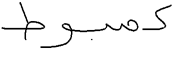
\includegraphics[width=0.2\textwidth]{./figures/kmbot_black}
        }
        \subfloat[]{
           \label{fig:kmbot_color}
           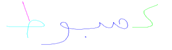
\includegraphics[width=0.2\textwidth]{./figures/kmbot_color}
        }        
    \caption{
        The Tunisian city name kambot. As can be seen in (b) it contains two word parts (KKRL{kmbw} and  KKRL{.t}). The main body of the first word part is written in 2 strokes (KKRL{k-} and KKRL{-mbw}). The second WP contains only a single letter (KKRL{.t}) and is written using 2 strokes, the main body and an additional stroke.   
     }
   \label{fig:kmbot}
\end{figure}

\begin{figure}[h]
\centering
        \subfloat[]{
            \label{fig:letters_same_body_1}
            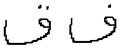
\includegraphics[width=0.2\textwidth]{./figures/letters_same_body_1}
        }
        \subfloat[]{
           \label{fig:letters_same_body_2}
           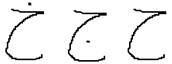
\includegraphics[width=0.2\textwidth]{./figures/letters_same_body_2}
        }        
    \caption{
        Letters groups having the same main body and only differ by their additional strokes
     }
   \label{fig:same_main_body_letters}
\end{figure}

In the analytic approach, character segmentation is a crucial part of the text recognition process. Correct segmentation of a word into letter is likely to result in a correct recognition. The recognition-based segmentation approaches the other way around is also valid, a good recognition system improves the segmentation precision. Several segmentation techniques have been proposed in the literature for Arabic OCR. However correct and efficient segmentation of Arabic text is still considered a challenging and a fundamental problem even for off-line printed text.  
[talk about over and under segmentation in the general case, not specifically to the Arabic]\\


Restricting our discussion to the analytic approach, the segmentation can be classified two main methods
\begin{itemize}
  \item Dissection
  \item Recognition Based Segmentation
\end{itemize}

Dissection techniques learn the characteristic of the segmentation point and try to find these features in a candidate point. For example, in English cursive script segmentation a common feature is that segmentation point has local minima in the upper or lower contour of the word. Another feature is the slope of the segmentation point is low. Some techniques don't try to segment a word to its letters but to graphemes, which are a combination of 2 or 3 letters or is a part of a letter. The recognition-based techniques operation is quite different. In principle no feature-based dissection algorithm is employed. Rather, the image is divided systematically into many overlapping pieces without regard to content. These are classified as part of an attempt to find a coherent segmentation / recognition result. The main interest of this category of methods is that they bypass the segmentation problem: no complex "dissection" algorithm has to be built and recognition errors are basically due to failures in classification. In recognition-based techniques, recognition can be performed by following either a serial or a parallel optimization scheme. In the first case recognition is done iteratively in a left-to-right scan of words, searching for a "satisfactory" recognition result. The parallel method proceeds in a more global way. It generates a lattice of all (or many) possible feature-to-letter combinations. The final decision is found by choosing an optimal path through the lattice [2]. A common approach that is followed by many researchers is over-segmentation of the text and validating each such candidate segmentation point by extracting feature vectors representing the segmented parts to some classifier or rules based engine.\cite{daifallah2009recognition}\\

In this paper we propose a novel approach which performs segmentation and recognition in the strokes level. We combine both holistic and analytic techniques for recognizing open dictionary Arabic on-line script. In section 2 we mention related Work done in the field of online Arabic recognition. In section 3, we describe the details of our approach. Results are displayed in the section 4. We discuss and conclude the work in section 5.
\\ \emph{Decorate the Introduction by citations]}

\subsection{Related Work}
A rules-based system for off-line Arabic handwritten word segmentation was presented by Abdulla et al. in \cite{abdulla2008off}. Their method is based on extracting features of pixels lying on the upper contour. The freeman chain coding scheme was used to find the coordinates of the contour. The slope of the upper contour pixels is calculated and the direction of pairs of adjacent coordinate were marked by ‘+’ or ‘-‘. Segments were combined to formulate bigger decisive segments (DS). Set of possible segmentation point are nominated from the ‘+’ marked segments. These segmentation points were evaluated using a certain rules to find the final segmentation points (FSP). The system was tested on the demo version of IFN/INIT described in \cite{pechwitz2002ifn} , and their own AHD/AUST database.\\

Randa et al. proposed a two stage word segmentation system of online Arabic handwritten text based on Hidden Markov Model (HMM) \cite{elanwar2012unconstrained}. In the first stage, segmentation points were nominated by a simultaneous segmentation-recognition method using HMM.  The proposed segmentation points were validated by a rules-based stage. Additional strokes were removed and not taken into consideration in both parts. The system was tested using a self-collected database (OHASD) that was described in \cite{elanwar2010ohasd}.\\

Sari et al. in their paper \cite{sari2002off} proposed a method for off-line Arabic Word parts segmentation, based on the topological characteristics of the word contour. They applied 8-connected contour following algorithm to achieve a smoothed sequence of the X-Y coordinates of the outer contour. Then, identified Local minima in the lower outer contour to nominate Segmentation points and then formulated a rules based engine to identify valid segmentation points. The system was evaluated using a small database that contained 100 handwritten Arabic words sampled.\\

Laslo Digness et al. in \cite{Dinges2011} proposed a segmentation based recognition approach for off-line Arabic Handwritten words. Their method is based on dividing the word to smaller pieces which afterwards segmented into candidate letters and then classified into letter classes using statistical and structural features. Decisive tree were used to reduce the number of potential classes; neural networks to compute weights for all statistical features the output of this process was used as input for a k-NN classifier.\\

Khaled Daifallah et al. in \cite{daifallah2009recognition} proposed a method for on-line Arabic handwritten words recognition. Their method operates on the stroke level. It established on segmentation-based recognition which contain several stages. The first stage proposes over-segmentation of the stroke. The segmentation points are selected by locating semi-horizontal lines moving from right to left. In a latter phase a portion of the segmentation points is filtered out by applying on a certain set of rules. Then HMM is used to classify the sub-strokes to letters using Hu feature. The candidate and its scoring letters are obtained. Based on tis results the set of best segmentation points are selected.   


\subsection{Approach}
Our approach employs both rules-based dissection and recognition-base segmentation techniques. The main idea of is to automatically segment a stroke while being scribed. A stroke is a subcomponent of a WP that spans from the pen down event to the corresponding pen up event. It may contain a single or multiple letters. We assume that each letter is contained entirely in a stroke, i.e. no letter span over multiple strokes. This assumption is valid for the majority of Arabic writing styles. The motivation behind this method is that only thing that needs to be really segmented is the stroke, and it is usually a standalone component, meaning that a reader can read what it contains. Thus being able to correctly segment and recognize the content of a stroke, cracks the Arabic script recognition problem. In this work our objective is to maximize the segmentation rate of Arabic handwritten words while maintaining low complexity and high performance of the system, rather than maximizing the recognition results. 
The proposed technique can be combined with any letters recognition system and post processing system to achieve a complete word level online recognition technique. The proposed scheme defines a general scheme for ongoing Arabic script recognition based segmentation and can be used with different letter recognition techniques. In the figure below we describe a high level architecture of a complete Arabic Handwritten Word/Word-part segmentation-based recognition system employing our proposed recognition based segmentation approach. 
  
\begin{figure}[h]
\centering
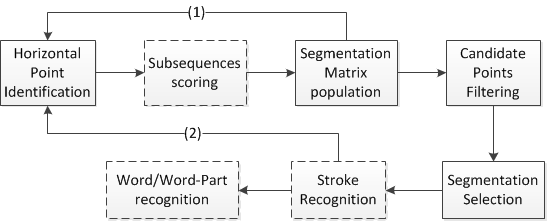
\includegraphics[width=9cm]{./figures/main_system_components}
\caption{Main System components}
\label{fig:main_system_components}
\end{figure}

The approach consists of several stages. 
\begin{description}
  \item[Stage 1] \hfill \\
  Ongoing Segmentation points nomination. Horizontal fragment (HF) identification. subsequences scoring calculation. Segmentation Scoring Matrix (SSM) construction. On every new Candidate point found, a new row and column are added to the matrix that contain the relevant subsequences scoring.
  \item[Stage 2] \hfill \\
  Redundant candidate points elimination and scoring correction.
  \item[Stage 3] \hfill \\
  Once the stroke is done (Pen Up Event). Segmentation points selection among the candidate points and. segmentation point selection algorithm is employed to select the most probable segmentation points.
\end{description}

\begin{figure}[h]
\centering
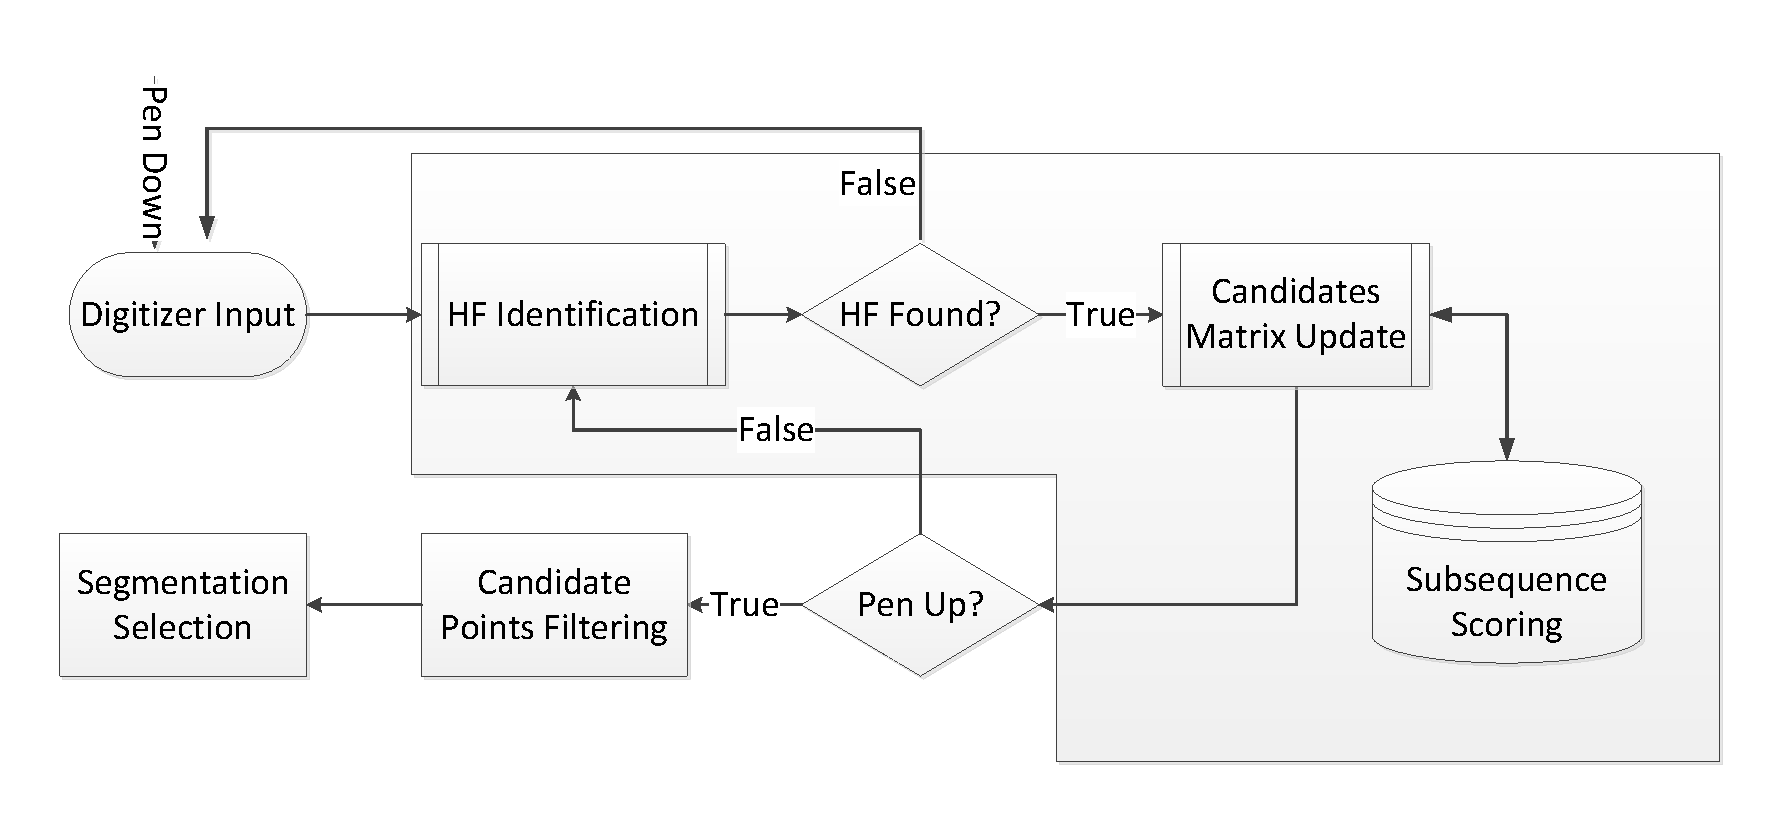
\includegraphics[width=9cm]{./figures/system_flow}
\caption{High level system flow}
\label{fig:system_flow}
\end{figure}

More details on every stage are provided in the subsections below.

\subsection{First Stage: Segmentation points nomination and sub-strokes scoring}

\subsubsection{Preprocessing}
In the on-line handwriting recognition, the data is obtained by a digitizer. Most classification method requires the data to admit to several properties, such as size, vector sample length, etc… The data obtained by the digitizer may not have these properties, since it is affected but the handwriting speed, hand vibration and digitizer imperfection. The preprocessing is performed to overcome this mismatches and normalize the data to have a uniform structure. In order to avoid digitizer noises, we have performed preprocessing operations that include simplification using Douglas simplification algorithm and re-sampling to achieve a smooth equidistant sample points. 
 
\begin{figure}[h]
	\centering
        \subfloat[]{
            \label{fig:letters_same_body_1}
            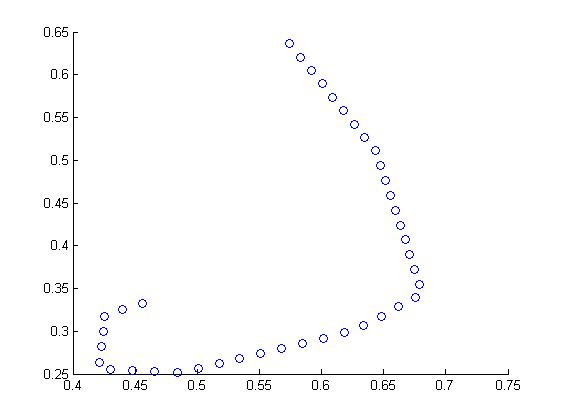
\includegraphics[width=0.2\textwidth]{./figures/letter_before_preprocessing}
        }
        \subfloat[]{
           \label{fig:letters_same_body_2}
           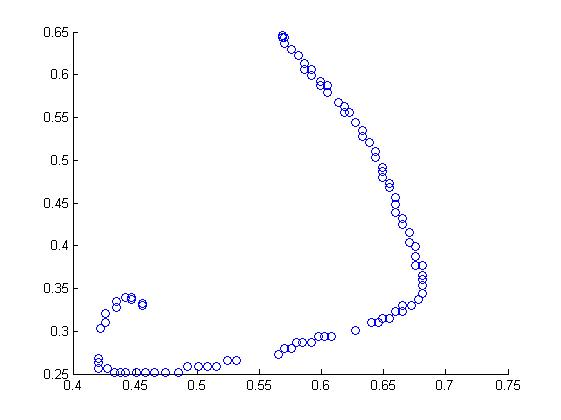
\includegraphics[width=0.2\textwidth]{./figures/letter_after_preprocessing}
        }        
    \caption{The letter KKRL{d} before (a) and after (b) preprocessing}
   \label{fig:same_main_body_letters}
\end{figure}

\subsubsection{Horizontal Fragment identification}

A stroke is represented by a sequence of points on the 2-dimensional space, $p_{i}=(x,y)$ 
\begin{equation}
S={p_{i}}_{i=1}^{n}
\end{equation}
Arabic segmentation points are usually contained in horizontal fragments (HF) of the stroke. In this stage such fragments are identified in the written text. Once an HF is detected, its medial point is set as a candidate point (CP). A HF is a subsequence of the stroke that is relatively straight, has a low slope and directed right to left. In the ongoing process to get the largest possible HF, we mark both the beginning and the end of the horizontal segment. 
A pair of adjacent points $\overline{p_{i}p_{i+1}}$ is considered horizontal if the its slope is low $\frac{\Delta y}{\Delta y}\leq0.6$ relative the horizontal axis i.e. $\phi \leq \frac{\pi}{6}$ . This parameter was found empirically and independently on \cite{daifallah2009recognition}. Who has found the same parameter. \\

A horizontal segment may contain a two points at least. We try to identify the largest possible HF. Ideally the whole process should be initiated on every new point received by the digitizer, however, it is unnecessary since no much information is obtained by each new point, we invoke the process on every k point, when k is one of the Parameters of the system and set to be 5 in our system.   

\begin{figure}[h]
\centering
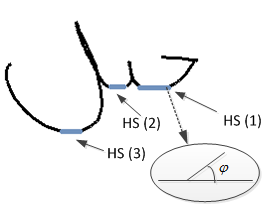
\includegraphics[width=6cm]{./figures/horizontal_segments}
\caption{Horizontal Segments [HS] of the word KKRL{jbl}(JABAL)}
\label{fig:horizontal_segments}
\end{figure}

\subsubsection{Sub-strokes scoring}
The candidate point $CP_{i}$ represents the index of the candidate point $i$ in the stroke $S$. For the simplicity of the presentation we define $CP_{i}=1$, i.e. the first point in the stroke $S$, although the first point is not defined as a segmentation point. We also we define the last point in the stroke $S$ as a candidate point, although it is not a candidate point but an obvious segmentation point. Both the "first candidate point" and the "last candidate point" will not be taken into account in the results sections.   

\begin{figure}[h]
\centering
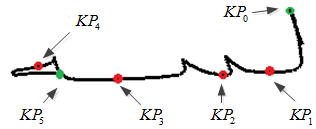
\includegraphics[width=9cm]{./figures/candidate_points}
\caption{Candidate points of the word  KKRL{lbyh}. The first and last candidate points are colored in green. The red points are the actual candidate points}
\label{fig:candidate_points}
\end{figure}

A sub-stroke $S_{i}^{j}$ is a sub-sequence of the stroke $CP_{i}$ that starts at candidate point $CP_{j}$ and ends at candidate point , i.e.
\begin{equation}
S_{i}^{j}=(p_{k})_{k=CP_{i}}^{CP_{j}}; i<j
\end{equation}

The sub-stroke  $S_{i}^{j}$ may represent a letter or a portion of a letter. In some cases it also may represent a multiple connected letters. The scores matrix $D\in\mathbb{R}^{nXn}$ contains the resemblance scoring for all sub-strokes. 
\begin{equation}
D(i,j)=Score(S_{i}^{j})
\end{equation}
Score($S_{i}^{j}$) is the classification scoring given by the letter classifier to the sub-stroke $S_{i}^{j}$. It is s clear that $D$ is an upper triangular matrix. For the sake of good performance as well as segmentation correctness we add a locality constraint to improve performance and to avoid marginal segmentation. That is, we only calculate a narrow band of the $D$ matrix above the diagonal. The band width is no larger than $L$.
\begin{equation}
D(i,j)=\inf if j \leq i or j-i>L 
\end{equation}

The matrix $D$ is calculated while the stroke is being scribed. Once a new candidate point is identified, a new row and column is added to the matrix with the corresponding Score($S_{i}^{j}$) for each added cell in the band of the lower triangular matrix. It can be easily noted that the number of cells calculates in the limited band is $O(LN)$ where $N$ is the number of candidate points in the stroke. 
A letters classifier that is described in depth in [my paper] is used to score the sub-strokes. For the sake of completeness, here we will outline the main idea of the classification system. The classifier uses Earth movers Distance embedding technique descried in \cite{shirdhonkar2008approximate} to project samples of the Arabic letters to a low dimensional space. Since the embedding is into the L1 space, given a sequence, the k-NN are found using k-dtree. The exact resemblance score is determined by a minimum score that is given by a predefined linear combination of the $L_{1}$ distance in the embedding space and Sokoe-Chuba DTW.

The classifier receives a sequence and a position, and it contains 4 databases; each database contains letter samples in a certain position (Ini, Mid, Fin or Iso) regardless of the letter label. As mentioned before a stroke can contain a single or several letters. Here we enumerate all the letters positions options that a stroke can contain.  

\begin{multicols}{2}
\begin{itemize}
    \item $Ini$
    \item $Mid^{+}$
    \item $Fin$
    \item $Ini,Mid^{*},Fin$
    \item $Ini,Mid^{+}$
    \item $Mid^{+},Fin$
\end{itemize}
\end{multicols}
Where $^+$ represent more than one occurrence and $^*$ represents zero or more occurrences. The $D_p$ matrix below demonstrates the databases in which the classifier will look into when trying to find the closest candidates. In Equation \ref{dp_matrix}, the Greek letter represents the set of position databases that the sub-stroke may belong to:

\begin{equation}
D_{p}=
\left( \begin{array}{cccccc}
\infty & \alpha & \alpha & \alpha & \cdots & \delta \\
\infty & \infty & \beta & \beta & \cdots & \chi \\
\infty & \infty & \alpha & \beta & \cdots & \chi \\
\infty & \infty & \infty & \infty & \cdots & \chi \\
\vdots & \vdots & \vdots & \vdots & \ddots & \vdots \\
\infty & \infty & \infty & \infty & \cdots & \infty \end{array} \right)
\label{dp_matrix}
\end{equation}

\begin{multicols}{2}
\begin{itemize}
    \item[] $\alpha=\{Ini\,or\,Mid\}$
    \item[] $\beta=\{Mid\}$
    \item[] $\chi=\{Mid\,or\,Fin\}$
    \item[] $\delta=\{Iso\,or\,Ini\,or\,Mid\,or\,Fin\}$
\end{itemize}
\end{multicols}

As mentioned before, for each subsequence, the recognition system returns a set of 3 potential letters candidates, with their resemblance scoring. In the current implementation we consider only the candidate with the best (minimal) scoring . In a future work we can evaluate other scoring technique that will be based on other scoring technique that will take into consideration all the relevant candidates.
In figure 5 and table [] we demonstrate the idea of the segmentation points nomination and the Subsequences matrix.
Table [] visually demonstrates the subsequences of the word shown in the figure above. Note that we have eliminated the first column and the last row of the matrix since it contains no subsequences.

\begin{figure}
\def\tabularxcolumn#1{m{#1}}
%\begin{tabularx}{\linewidth}{@{}cXX@{}}
\begin{tabular}[h]{| c |c | c | c| c | c | c |}
\hline
 & $CP_{1}$ & $CP_{2}$ & $CP_{3}$ & $CP_{4}$ & $CP_{5}$ & $CP_{6}$\\ 
\hline
$CP_{1}$
   & N/A
   & \subfloat{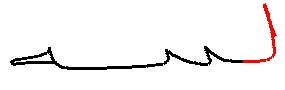
\includegraphics[width=0.8cm]{./figures/substrokes/L}}
   & \subfloat{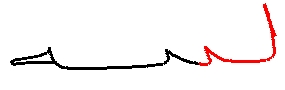
\includegraphics[width=0.8cm]{./figures/substrokes/LB1}}
   & \subfloat{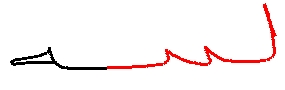
\includegraphics[width=0.8cm]{./figures/substrokes/LB1B2}}
   & N/A & N/A \\
\hline
$CP_{2}$
   & N/A & N/A
   & \subfloat{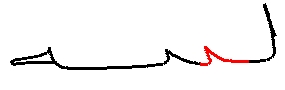
\includegraphics[width=0.8cm]{./figures/substrokes/B1}}
   & \subfloat{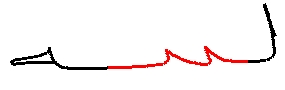
\includegraphics[width=0.8cm]{./figures/substrokes/B1B2}}
   & \subfloat{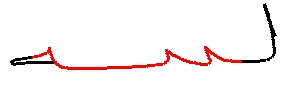
\includegraphics[width=0.8cm]{./figures/substrokes/B1B2H1}}
   & N/A \\
\hline
$CP_{3}$
   & N/A  & N/A & N/A
   & \subfloat{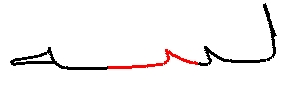
\includegraphics[width=0.8cm]{./figures/substrokes/B2}}
   & \subfloat{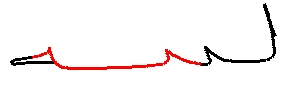
\includegraphics[width=0.8cm]{./figures/substrokes/B2H1}}
   & \subfloat{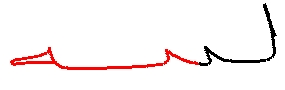
\includegraphics[width=0.8cm]{./figures/substrokes/B2H}} \\
\hline
$CP_{4}$
   & N/A & N/A & N/A & N/A
   & \subfloat{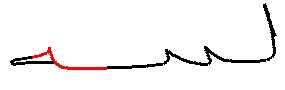
\includegraphics[width=0.8cm]{./figures/substrokes/H1}}
   & \subfloat{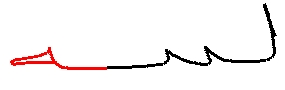
\includegraphics[width=0.8cm]{./figures/substrokes/H}} \\
\hline
$CP_{5}$
   & N/A & N/A & N/A & N/A & N/A
   & \subfloat{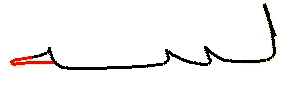
\includegraphics[width=0.8cm]{./figures/substrokes/H2}}\\
\hline
$CP_{6}$
   & N/A & N/A & N/A & N/A & N/A & N/A \\
\hline
\end{tabular}
%\end{tabularx}
\caption{Visual demonstration of subsequences of the word shown in figure \ref{fig:candidate_points}}
\label{table:substrokes_demo}
\end{figure}

\subsection{Second  Stage: Candidate points sieving and scoring correction}
In this stage we eliminate redundant segmentation points. The elimination is based on the following rules:

\begin{itemize}
\item [Rule 1]:	Inner Segmentation point lies close to the baseline. 
\item [Rule 2]:	Segmentation points do not reside in loops.
\item [Rule 3]:	A sub-stroke length/area is proportional to the stroke/length of the containing stroke.
\end{itemize}

The first is based on the fact that segmentation point lies on the baseline (see []), thus points that are mainly far from the baseline are eliminated. The baseline is proved to be an important piece of information in both segmentation and recognition domains of both on-line and off-line handwriting recognition. In words recognition, it plays a role in determining if an additional stroke to differentiate between diacritic dots according to their position from the baseline (above or under).
The second rule is clear since in most writing styles, segmentation point do not reside inside a loop.
The third rule's goal is to avoid high scoring resulted for discordant scaling of the letters; a scoring correction should be employed. It aims to reduce the effect of scaling problem. To illustrate the discordant scaling problem, see figure below. The suffix of the letter KKRL{d} is very similar to the letter KKRL{-a}. The only way to visually discriminate between them is by comparing the scaling of this suffix to the whole stroke dimensions. Thus this phase refines the recognition results according the subsequence scale in accordance to the sequence scale. We have penalized sub-strokes that are disproportional to the stroke size by multiplying the score of each sub-stroke with a Gaussian normalized by the stroke area/Length.
In some cases candidate segmentation points are incorrectly nominated on areas that are not horizontal, this is caused from the fact that the nomination is done while the word is being scribed, and our filtering algorithm should be corrected to handle this case.

\begin{figure}[h]
\centering
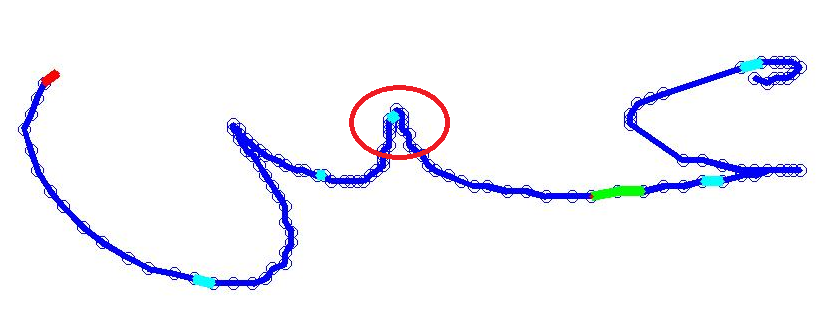
\includegraphics[width=9cm]{./figures/candidate_in_no_horizontal}
\caption{Incorrect nomination of a candidate point that lays on a Segmentation fragmnet.}
\label{fig:candidate_in_no_horizontal}
\end{figure}


In several cases we encountered candidate points that reside on the same horizontal fragment. [why does it happen?]. We filter out this redundant candidate points in the nomination process and do not wait till this filtering phase. The reason is that since we calculate a narrow band of the Scoring matrix, leaving the impermissible candidate points will result in low performance since highly over segment the word will cause also the system to miss letters because we calculate only a portion a narrow band of the scoring matrix. If such case is identified by the nomination algorithm the medial point between the adjacent candidate points is taken.

\subsection{Third  Stage: Segmentation Selection}
The goal of this phase is to select the best segmentation points set among the candidate segmentation points. It is done by finding the best segmentation path in $D$.
A path with the length in the scoring matrix $D^{mXn}$ is defined as follows:  
\begin{enumerate}
\item First link: $p_{1}=(1,j)$
\item $p_{k}=(i,j)\Rightarrow p_{k+1}=(j,r);s.t.:r>j \forall 1<k<l $
\item Last link: $p_{l}=(1,n)$
\end{enumerate}
Three algorithms are proposed in this work. The first we name as “Forward Segmentation Selection” (FSS) and the other is named the “Backward Segmentation Selection” (BSS) and the third named “Greedy Segmentation Selection” (GSS). The final segmentation is the segmentation that has the minimal between the FSS and BSS and GSS normalized by the number of Segmentation points. In the algorithm below, is the set of candidate points Including the pen-down point.  

\begin{figure}
\begin{algorithmic}
\STATE $i=1$
\STATE $sum=0$
\WHILE{$i<|CS|$}
\STATE $j = \mathop {\arg \min }\limits_k \left( {D\left( {i,k} \right)} \right)$
\STATE $FSS = FSS \cup \left\{ j \right\}$
\STATE $sum = sum + D\left( {i,j} \right)$
\STATE $i=j$
\ENDWHILE
\end{algorithmic}
\caption{Forward Segmentation Selection (FSS)}
\label{alg:fss}
\end{figure}

\begin{figure}
\begin{algorithmic}
\STATE $j={CS|}$
\STATE $sum=0$
\WHILE{$i<|CS|$}
\STATE $j = \mathop {\arg \min }\limits_k \left( {D\left( {k,j} \right)} \right)$
\STATE $BSS = BSS \cup \left\{ i \right\}$
\STATE $sum = sum + D\left( {i,j} \right)$
\STATE $j=i$
\ENDWHILE
\end{algorithmic}
\caption{Backward Segmentation Selection (BSS)}
\label{alg:bss}
\end{figure}

The idea in the following algorithm, is that in each iteration two segmentation point are selected, the first is the best score candidate point from the end of the stroke and the second is the best from the beginning. In this approach, it is less likely to step over segmentation point, like what happened in the FSS and BSS.

\begin{figure}
\begin{algorithmic}
\STATE $p_{a}=1$
\STATE $p_{b}=|CS|$
\STATE $sum=0$
\STATE $SSP=\{p_{a},p_{b}\}$
\WHILE{$SP \neq \emptyset$}
\STATE $p_{a,next} = \mathop {\arg \min}\limits_k (D(p_{a,next},k))$
\STATE $SSP = SSP \cup \{p_{a,next}\}$
\STATE $sum = sum + D(p_a,p_{a,next})$
\STATE Remove all cells that represent a candidate point that has an index lower than $p_{a,next}$
\STATE $p_{a}=p_{a,next}$
\STATE $p_{b,next} = \mathop {\arg \min}\limits_k (D(k,p_{b,next}))$
\STATE $SSP = SSP \cup \{p_{b,next}\}$
\STATE $sum = sum + D(p_{b,next},p_b)$
\STATE Remove all cells that represent a candidate point that has an index larger than  $p_{b,next}$
\STATE $p_{b}=p_{b,next}$
\ENDWHILE
\end{algorithmic}
\caption{Backward-Forward Segmentation Selection (BFSS)}
\label{alg:bfss}
\end{figure}

\begin{figure}
\begin{algorithmic}
\STATE $i={1}$
\STATE $SP=\emptyset$
\WHILE{$SP \neq \emptyset$}
\STATE $p_{a,next} = \mathop {\arg \min}\limits_k (D(i.j))$
\STATE $SSP = SSP \cup \{s,e\}$
\STATE $sum = sum + D(s,e)$
\STATE	Remove all cells that represent a candidate point between $CP_{i}$ and $CP_{j}$.
\ENDWHILE
\end{algorithmic}
\caption{Greedy Segmentation Selection (GSS)}
\label{alg:gss}
\end{figure}

In GSS, in every iteration, the cell with the best scoring is selected thus the selected cell represents a sub-sequence that has the best resemblance for a letter, thus this subsequence must be included in the final segmentation. If cell $D(i,j)$ was selected, both the candidate point $CP_{i}$ and $CP_{j}$ is added to the final set and every segmentation point between $i$ and $j$ are removed from the scoring matrix.

\section{Validation}
In this works, usually a human taken place to make sure that the segmentation is correct. In this paper, we have used an automatic validation process. For each segmentation point found by our system, for it to be count as a true positive, the information measure between the real segmentation point (marked by an expert human) and the segmentation point sound by the system should be small.

\subsection{Subsequence Complexity measure }
The aim of this measure is to give a numerical confidence that if two points reside on the relatively same straight line over the stroke. To demonstrate the idea see figure below. From another point of view, it can be thought about as the amount of information stored in a sub-sequence or the complexity of the sequence. This notion is used in 2 places in our work:
\begin{itemize}
\item The Horizontal fragment identification.
\item In the segmentation point validation step.
\end{itemize}

To calculate the complexity measure of a sequence, first we simplify the subsequence. Then, for each angle  $\phi=\angle(\overline{p_{i-1}p_{i}},\overline{p_{i}p_{i+1}})$ we calculate the parameter $\alpha_{i}$.
\begin{equation}
 alpha_{i}=\frac{\pi-\theta_{i}}{\frac{\pi}{6}}
\end{equation}
The complexity measure is the defined as:
\begin{equation}
CM(S)=\Sigma_{i}\alpha_{i}
\end{equation}

\begin{figure}[h]
     \begin{center}
        \subfloat[sequence 1]{
            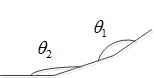
\includegraphics[width=0.2\textwidth]{./figures/angles_1}
        }
        \subfloat[sequence 2]{
           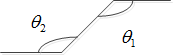
\includegraphics[width=0.2\textwidth]{./figures/angles_2}
        }        
    \end{center}
    \caption{A graphical representation of the angles of a sequence. It can be seen that per our definition Sequence 1 Complexity measure is smaller than sequence 2 complexity measure.}
   \label{fig:sequence_complexity}
\end{figure}

\section{The Database}
The data is the most important part of any supervised learning technique. The data is used for both learning, validation and testing stages and has a critical effect on the system performance. In this work we have chosen to use the ADAB database. The ADAB database is de-facto a standard in the on line Arabic handwriting recognition research field. It is freely available and consists of more than 20k Arabic handwritten words scribed by more than 170 different writers. The words are taken from the 937 Tunisian town/village names. It contains the trajectory information and a plot image of the word trajectory. The ADAB-database v.1 is divided to 3 sets. Details about the number of files, words, characters, and writers are detailed in [6]. Our training and testing set both are taken from this database. 
The information in the ADAB database provides for each word its label and the strokes that were written by the writer, no information relating the strokes to letters or to word parts provided, thus, some work needed to be performed to add this information to the database. This edition is needed for providing letters samples for our classifier as well as for being able to automatically evaluate the segmentation rate. We have created a friendly UI system that reads the samples in the ADAB database, and a human professional segment the samples. The output of this process is an xml for each word sample that contain letter level information, and WPs level details. Since additional strokes are not our interest in the segmentation process, the system automatically filtered out additional strokes. The professional had the ability to filter our additional strokes that could not be identified by the system as such. We have manually segmented ~8k samples which consisted about ~20k strokes.
Our system reads an xml files, extracts the strokes and information we provided our training system with letters and also extracted strokes to test our system. 

\section{Experimental Results}
Our system was implemented in Matlab environment. The total number of samples in the test set is 200. As mentioned a sample is a Tunisian city name, a city name can contain 1 or more words. 
Although our approach segments the written script in the stroke level, it is more reasonable to display the results in the WP and word levels. A correct segmentation of a word-part means that all the strokes of the in it were segmented correctly. A correctly segmented stroke is the case when all the letters in the stroke are correctly segmented.  In table 1 below, you can see the length distribution of the Word parts in the test set. By length we mean the number of letters the word part contains.
The segmentation points results were validated automatically, if a word part was recognized correctly that means that the segmentation is correct. For each letter we select the 3 letter and shoe our recognition results based on if one of the candidate letters is the correct letter.


\begin{table}[h]
\caption{Segmentation Points Results}
\begin{tabular}{ | c | c | }
  \hline                     
   Precision & 95.4\% \\ 
 \hline
  Recall &  95.6\% \\ 
 \hline
  Letters Recognition rate & 87.27\% \\
\hline
\end{tabular}
\centering
\label{table:sp_results} 
\end{table}
If the recognition was incorrect, each segmentation point recognized by the system was validated automatically by making sure that there is no much information between the segmentation ground truth and the segmentation provided by the system.

\begin{table}[h]
\caption{Word-Parts Results}
\begin{tabular}{ | c | c | }
  \hline                     
    Total Number of Word Parts & 197 \\ 
  \hline
  Segmentation Rate &  87.7\% \\ 
 \hline
  Recognition Rate &  70.94\% \\ 
 \hline
  Average Time & 0.64 [sec] \\
\hline
\end{tabular}
\centering
\label{table:wp_results} 
\end{table}

\begin{table}[h]
\caption{Distribution of WP length}
\begin{tabular}{ | c | c | }
  \hline                     
    1 & 25 \\ 
  \hline
  2 &  171 \\ 
 \hline
 3 & 136 \\ 
 \hline
  4 and more & 91 \\
\hline
\end{tabular}
\centering
\label{table:wp_length_dist} 
\end{table}

\subsection{Analysis}

\subsubsection{Over-segmentation}

To avoid a candidate point nomination in a horizontal fragment at the beginning of the stroke which is in most cases a false candidate point, we have added the limitation that segmentation point is nominated only if the sub-stroke that spans from the beginning of the stroke to the current point, is complex.
\begin{figure}[h]
\centering
        \subfloat[]{
            \label{fig:letters_same_body_1}
            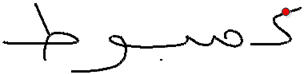
\includegraphics[width=0.3\textwidth]{./figures/oversegmentation_begin_1}
        }
        \subfloat[]{
           \label{fig:letters_same_body_2}
           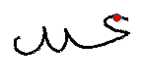
\includegraphics[width=0.15\textwidth]{./figures/oversegmentation_begin_2}
        }        
    \caption{Samples of redundant Candidate point at the beginning of the  stroke.}
   \label{fig:oversegmentation_begin}
\end{figure}

\begin{figure}[h]
\centering
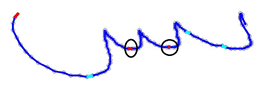
\includegraphics[width=5cm]{./figures/oversegmentation_s}
\caption{Over-segmentation in the letter س. These happens since this letter is very similar to the appearance to a combination of two consequtive ب (ـببـ) letters and only can be identified from the context and using the additional strokes }
\label{fig:oversegmentation_s}
\end{figure}

\begin{figure}[h]
\centering
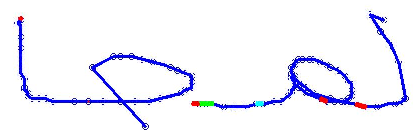
\includegraphics[width=5cm]{./figures/oversegmentation_m}
\caption{Over-segmentation appeared frequently in the letter M, since it contains two horizontal segments (can be handled by eliminatinf candidate points in a loop).}
\label{fig:oversegmentation_m}
\end{figure}

\subsubsection{Under-segmentation}
It may results from 2 reasons:

\begin{enumerate}
\item No point is get nominated in the horizontal fragment
\item Nominated but not selected.
\end{enumerate}

The first mainly results from letter pairs that do not contain horizontal joint between them; this issue is partially solved by extending the notion of a letters to include such pairs of letters. For example the pair لم and لح, these letters may have 2-4 positions. The second may result from nomination of a candidate point on correct horizontal segment but in a late fraction of the segmentation fragment which result is a low scoring and thus not being selected by the Segmentation selection algorithm. This issue usually occurs in the letter و in its final position.

\begin{figure}[h]
\centering
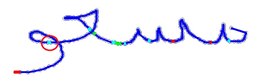
\includegraphics[width=5cm]{./figures/undersegmentation_w}
\caption{An example of a late candidate point in the letter و.}
\label{fig:undersegmentation_w}
\end{figure}


\begin{table}[h]
\caption{Performance of each Segmentation selection algorithm}
\begin{tabular}{ | c | c | c | }
Segmentation Selection Algorithm & WP Segmentation Rate & WP Recognition Rate	  \\
\hline                 
  FSS & 81.5\% & 70.9\% \\ 
  \hline
  BSS & 78.4\% &  37.5\% \\ 
 \hline
 GSS & 77.1\% & 68.7\% \\ 
 \hline
  FBSS & 83.34\% & 73.74\% \\
\hline
\end{tabular}
\centering
\label{table:ss_algorithms_results} 
\end{table}

Most error in the final segmentation is caused by segmentation selection algorithm. Thus we had to combine several segmentation selection approaches to achieve the best results.
We will show that the maximal number of letters does not affect much the segmentation rate and recognition rate, the graph will convergence after 200 samples per letter.

\begin{figure}[h]
\centering
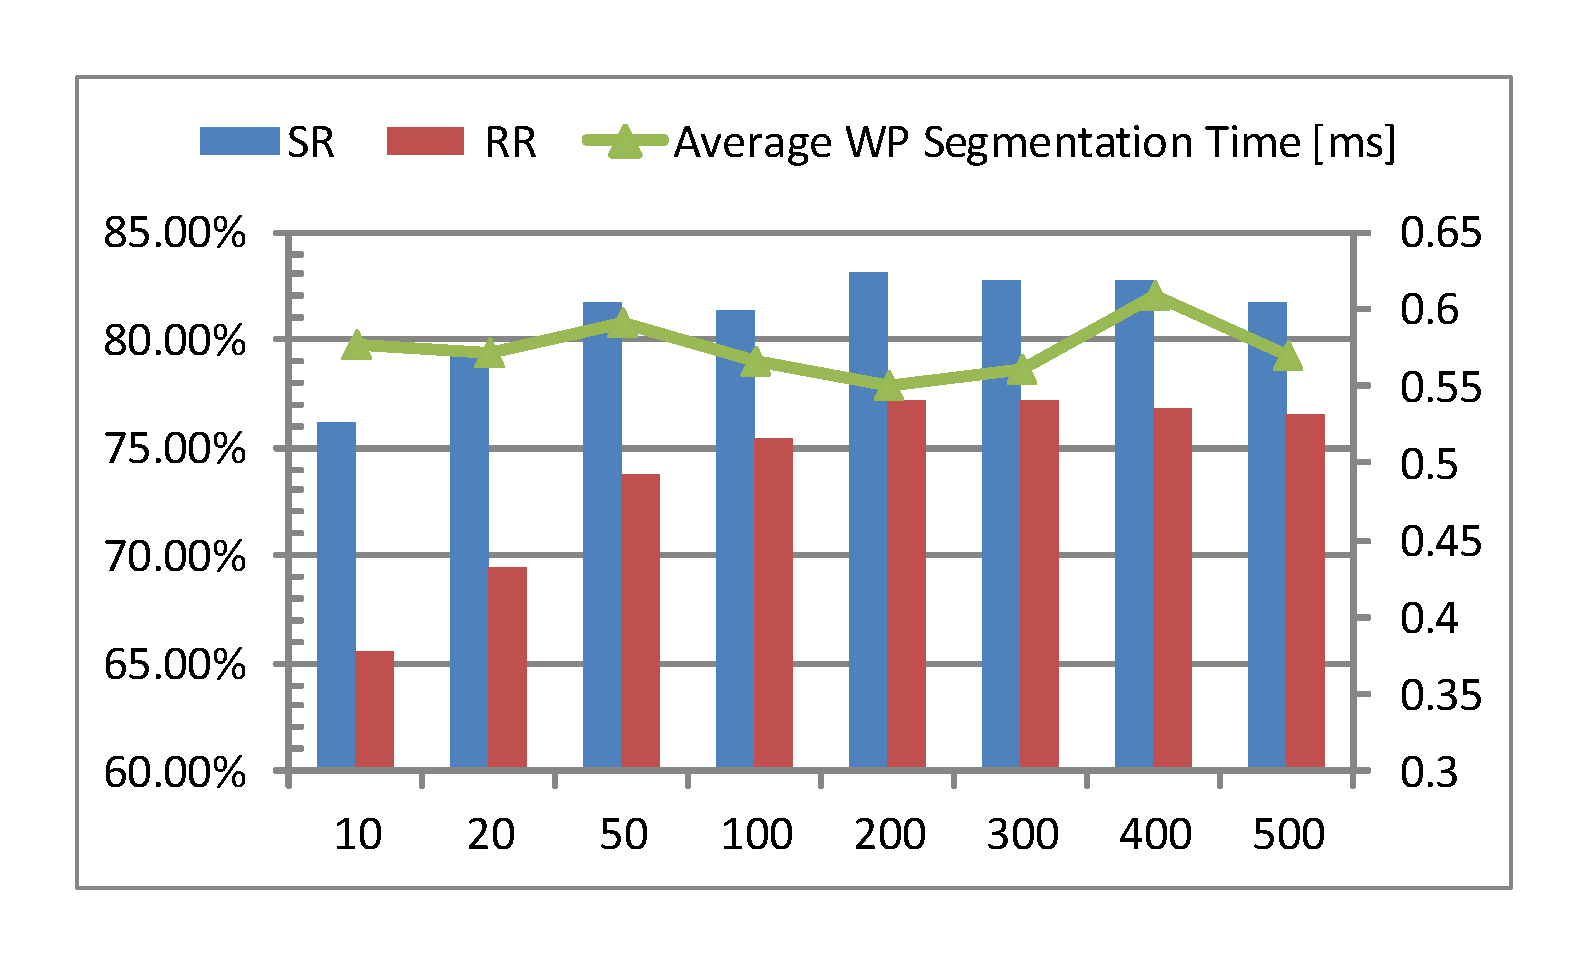
\includegraphics[width=9cm]{./figures/num_letter_impact}
\caption{The diagram shows the influence of the number of letters samples on the segmentation (SR) , recognition rates (RR) , and the average segmentation time. All the three parameters showing convergence when the maximum letter samples per letter position is larger than 200. }
\label{fig:num_letter_impact}
\end{figure}


\section{Future Work}
[we can fix the orientation problem in figure work by rotating by different angles but the ADAB sample are our system could easily handle samples to]

[Consider the delayed strokes segmentation: every strokes is classified to be in the main body or an additional stroke, id classified in the main body, then we handled it. If classified as a delayed stroke, it should be matched to the letter is related.
For every word, the key a serious of features such that
(A,Ham, KL): أكل
(D,Dot,HB): ذهب


\bibliographystyle{IEEEtran}
\bibliography{IEEEabrv,bibliography}

\end{document}


